\documentclass[conference]{IEEEtran}
\IEEEoverridecommandlockouts
% The preceding line is only needed to identify funding in the first footnote. If that is unneeded, please comment it out.
\makeatletter
\def\endthebibliography{%
	\def\@noitemerr{\@latex@warning{Empty `thebibliography' environment}}%
	\endlist
}
\makeatother
\usepackage{cite}
\usepackage{amsmath,amssymb,amsfonts}
\usepackage{algorithmic}
\usepackage{hyperref}
\usepackage{graphicx}
\usepackage{textcomp}
\usepackage{xcolor}
\usepackage{adjustbox}
\usepackage{multirow}
\usepackage{subcaption}

\usepackage{float}
\usepackage[shortlabels]{enumitem}


\def\BibTeX{{\rm B\kern-.05em{\sc i\kern-.025em b}\kern-.08em
		T\kern-.1667em\lower.7ex\hbox{E}\kern-.125emX}}
\begin{document}
	
	\title{ITS Autonomous Car Maneuver at Roundabouts or U-Turn using Deep Reinforcement Learning}
	
	\makeatletter
	\newcommand{\linebreakand}{%
	\end{@IEEEauthorhalign}
	\hfill\mbox{}\par
	\mbox{}\hfill\begin{@IEEEauthorhalign}
	}
	\makeatother
	
	\author{
		\centering
		
		\IEEEauthorblockN{1\textsuperscript{st}Prof. Dr. Ir. Mauridhi Hery Purnomo, M.Eng.}
		\IEEEauthorblockA{\textit{Department of Computer Engineering} \\
			\textit{Faculty of Intelligent Electrical}\\
			\textit{and Informatics Technology}\\
			\textit{Institut Teknologi Sepuluh Nopember}\\
			Surabaya, Indonesia 60111 \\
			hery@ee.its.ac.id}
		\and
		\IEEEauthorblockN{2\textsuperscript{nd}Dr. I Ketut Eddy Purnama, ST., MT.}
		\IEEEauthorblockA{\textit{Department of Computer Engineering} \\
			\textit{Faculty of Intelligent Electrical}\\
			\textit{and Informatics Technology}\\
			\textit{Institut Teknologi Sepuluh Nopember}\\
			Surabaya, Indonesia 60111 \\
			ketut@ee.its.ac.id}
		\and
		\IEEEauthorblockN{3\textsuperscript{nd}Muhtadin, ST., MT.}
		\IEEEauthorblockA{\textit{Department of Computer Engineering} \\
			\textit{Faculty of Intelligent Electrical}\\
			\textit{and Informatics Technology}\\
			\textit{Institut Teknologi Sepuluh Nopember}\\
			Surabaya, Indonesia 60111 \\
			muhtadin@te.its.ac.id}
		\and
		\IEEEauthorblockN{4\textsuperscript{rd} Muhammad Roychan Meliaz}
		\IEEEauthorblockA{\textit{Department of Computer Engineering} \\
			\textit{Faculty of Intelligent Electrical}\\
			\textit{and Informatics Technology}\\
			\textit{Institut Teknologi Sepuluh Nopember}\\
			Surabaya, Indonesia 60111 \\
			meliaz.17072@mhs.its.ac.id}
		
	}
	
	\maketitle
	
	
	\begin{abstract}
		\textit{An autonomous car or autonomous vehicle is a vehicle
		which has the ability to drive independently as if controlled by humans using a series of artificial intelligence. In this study, we propose research on the development of an autonomous vehicle iCar ITS (Intelligent Car Institut Teknologi Sepuluh Nopember) by developing a maneuvering system for autonomous vehicles at roundabouts or u-turns in a simulated environment. In the simulation environment, the model used is a vehicle model adapted to iCar. The development of autonomous vehicle navigation and maneuvering systems is carried out using the Deep Reinforcement Learning method, a branch of Machine Learning. From this research, the results obtained are reinforcement learning models that are able to maneuver at roundabouts with intersections and roundabouts without intersections with a mean deviation value of the angle of the path of 27,011° and 30,068°, respectively, able to maneuver without collision for an average of 13.3 seconds and 7.9 seconds, and with an average speed of 27.0 kmph and 28.5 kmph.}
	\end{abstract}
	\begin{IEEEkeywords}
		\textit{Autonomous Vehicle, Reinforcement Learning, Deep Learning, Simulation}
	\end{IEEEkeywords}
	
	\section{Introduction}
	\IEEEPARstart{A}{utonomous} vehicle technology has a long history. The first fully functional prototype was built in 1980. Using a camera, this prototype managed to cover 100km of empty roads without needing to be steered by humans. With this success came many projects in the 80s and 90s using similar systems used for driving through highways, in either light or no traffic. In its development, autonomous vehicles can solve the problem of driving safety and efficiency. Therefore, the main objective of the research is to prevent or reduce traffic accidents, reduce the time people drive, and reduce carbon emissions.\cite{cit:autonomous_vehicle_future}\par
	
	One of the autonomous car products being developed is iCar ITS (Intelligent Car Institute of Technology Ten November). iCar ITS is a prototype car equipped with autonomous driving features as a result of collaborative research from ITS researchers with various fields of expertise.\cite{cit:icar_menristekbrin} iCar ITS is operated as a commuter car that serves passenger trips to various destinations within the ITS campus.\cite{cit:icar_its_news}
	
	
	A commonly used method for developing autonomous vehicles is reinforcement learning, a subset of machine learning that is also a subset of artificial intelligence. Reinforcement Learning is a learning method about what to do (implement actions into situations) on a problem/problem to get maximum results/reward. Agents are not given instructions on what actions to take. Agent will take action with the principle of Trial and Error, then make a decision based on the reward obtained (maximum reward).
	
	In its application, iCar ITS still uses the traditional rule-based method without utilizing machine learning methods. This method is not good enough because the developer has to manually program every scenario that the iCar will face. This method will not last long given the number of real-world scenarios that are almost impossible to solve manually.
	
	\section{System Design and Implementation}
	\vspace{1ex}
	This section describes the application of the Deep Reinforcement Learning method which aims to create an algorithm for an autonomous car capable of efficiently maneuvering roundabouts or u-turns.
	
\subsection{Simulation Environment Preparation}
\label{sec:simulasi}
Using the CARLA simulator, the Town03 CARLA map is used, which has a roundabout and a u-turn to facilitate research work. There are two types of roundabouts used in this study.

\subsubsection{Roundabout with Intersections}
The four-way roundabout is used as shown in Figure \ref{fig:bundaran_town03}. In this environment, the agent will spawn from four spawn points around the roundabout.
\begin{figure}[H] 
	\centering
	\includegraphics[width=1\linewidth]{images/bundaran}
	\caption{Roundabout with Intersections}
	\label{fig:bundaran_town03}
\end{figure}

\subsubsection{Roundabout without Intersection}
A roundabout without an intersection is used as shown in Figure  \ref{fig:bundaran_tanpa_simpang}. In this environment, the agent will spawn from an initial spawn point of the roundabout.
\begin{figure}[H] 
	\centering
	\includegraphics[width=1\linewidth]{images/bundaran_tanpa_simpang}
	\caption{Roundabout without Intersection}
	\label{fig:bundaran_tanpa_simpang}
\end{figure}

\subsection{Sensors}
\label{sec:sensor}
In this study, a camera sensor is used which is physically placed on the lower front of the agent. The camera sensor used is a segmentation camera sensor. The segmentation camera sensor is a camera sensor that separates objects in the simulator into a variety of unique solid colors. The image generated from the segmentation camera sensor in Figure  \ref{fig:segmentasi} is an advanced image that has been processed from the RGB image in Figure \ref{fig:citra_rgb}


\subsection{Data Acquisition}
\label{sec:akuisisi_data}
Image data is taken from the sensor with a size of 480x270. The image used is a segmented image that has been provided by the segmentation camera sensor from the CARLA Simulator. Seen in Figure \ref{fig:citra_rgb} is the initial image. Then segmentation is carried out on the image so that each object is presented with a solid color as shown in Figure \ref{fig:segmentasi}

\begin{figure}[H] 
	\centering
	\includegraphics[width=1\linewidth]{images/rgb}
	\caption{RGB Image}
	\label{fig:citra_rgb}
\end{figure}
\begin{figure}[H] 
	\centering
	\includegraphics[width=1\linewidth]{images/segmentasi}
	\caption{Segmented Image}
	\label{fig:segmentasi}
\end{figure}
There are two types of images used in this study, namely grayscale segmentation images and advanced segmentation images.

Grayscale segmentation image is a segmented image which is then given a grayscale filter in order to minimize the analyzed data but still maintain the existing features.	

\begin{figure}[H] 
	\centering
	\includegraphics[width=1\linewidth]{images/grayscale}
	\caption{Citra Segmentasi Grayscale}
	\label{fig:grayscale}
\end{figure}

The advanced segmentation image is a segmented image, which is then re-segmented into two types of objects, namely drivable and non-drivable. Drivable objects are represented in white and non-drivable objects are represented in black.

\begin{figure}[H] 
	\centering
	\includegraphics[width=1\linewidth]{images/segmentasi_hitam_putih}
	\caption{Citra Segmentasi Lanjutan}
	\label{fig:segmentasi_hitam_putih}
\end{figure}

Grayscale segmentation images and advanced segmentation images will be the final result of image acquisition which will then be given to the DQN algorithm to perform model training and/or inference models.

\subsection{\textit{Action}}
\label{sec:action}
There are 3 actions that the agent can take. Among them are:

\begin{enumerate}
	\item \verb=forward=
	
	Agent throttle with a value of 1 and steer with a value of 0. Thus the agent will perform a forward maneuver.
	
	\item \verb=forward_left=
	
	Agent throttle with a value of 1 and steer with a value of -1. Thus the agent will perform a forward left maneuver.
		
	\item \verb=forward_right=
	
	Agent throttle with a value of 1 and steer with a value of 1. Thus the agent will perform a forward right maneuver.
		
\end{enumerate}

\subsection{\textit{Reward Function}}
\label{sec:sistem_reward}

The reward function is designed to allow autonomous cars to move along the track quickly and safely.

\subsubsection{Roundabout with Intersections}There are four rewards set. Each reward pays attention to the reference lane target. The target lane is an imaginary line that is the target of the autonomous car movement. Seen in Figure  \ref{fig:target_lane_line}, the target lane is depicted with red dots around the roundabout.

\begin{figure}[H] 
	\centering
	\includegraphics[width=1\linewidth]{images/target_lane_line}
	\caption{\textit{Target lane}}
	\label{fig:target_lane_line}
\end{figure}

\begin{enumerate}[a)]
\item \textit{Reward} 1: Angle deviation from the target lane.
The reward used in Reward 1 is 1/alpha. Alpha is the angle of the agent that deviates from the target lane. The alpha technique is described in Figure  \ref{fig:reward_anglediff_sketch}. 

\begin{figure}[H] 
	\centering
	\includegraphics[width=1\linewidth]{images/reward_anglediff_sketch}
	\caption{Reward 1}
	\label{fig:reward_anglediff_sketch}
\end{figure}

The black line is a perpendicular vector from the center of the circle to the center of the agent. Then the red line is the direction vector of the car. From these two values, we get alpha which is the angle of the two vectors. Then the reward value is defined by 1/alpha. The highest reward value is limited to 1. This is done so that the fluctuation of the reward given to the agent is not too high for a small change in value.

\item \textit{Reward} 2: Distance deviation from the target lane.
The reward used in reward 2 is 1/distance\_deviation*10. Distance deviation is the agent's smallest distance from the target lane in meters.

\begin{figure}[H] 
	\centering
	\includegraphics[width=.85\linewidth]{images/reward_deviasi_jarak}
	\caption{Reward 2}
	\label{fig:reward_deviasi_jarak}
\end{figure}
The highest reward value is limited to 1. This is done so that the fluctuations in the reward given to the agent are not too high for a small change in value, as in Reward 1.


In addition to positive rewards, negative rewards are also needed to reduce the opportunity for agents to do things that should not be done. There are two negative rewards given.

\item \textit{Reward} 3: Collision with other objects.
A reward of -1 will be given to the agent if the agent touches other objects other than roads, ground, and sidewalks.

\item \textit{Reward} 4: Distance deviation too big.
A reward of -0.5 will be given to the agent if the distance between the agent and the roundabout is greater than 30 meters. The distance of 30 meters from the roundabout can be seen in Figure \ref{fig:punishment_lane_line}

\begin{figure}[H] 
	\centering
	\includegraphics[width=1\linewidth]{images/punishment_lane_line}
	\caption{Distance Limit}
	\label{fig:punishment_lane_line}
\end{figure}

\item{Total \textit{Reward }}
The total reward value is defined as Reward 1 + Reward 2 + Reward 3 + Reward 4.

\end{enumerate}


\subsubsection{Roundabout without Intersection}
At roundabouts without intersections, the reward function given is different. In this case, path points are provided as waypoints that the agent must follow.

\begin{figure}[H] 
	\centering
	\includegraphics[width=1\linewidth]{images/waypoint}
	\caption{\textit{Waypoint}}
	\label{fig:waypoint}
\end{figure}

Waypoints are points on the map as the target destination for the agent. Seen in Figure \ref{fig:waypoint}, the red dots are illustrations of waypoints. Waypoints are 100 physical points where each point is one meter apart.

\begin{enumerate}[a)]
\item \textit{Reward} 1: Angle deviation from \textit{waypoint}.
Rewards are defined by 1/alpha. Alpha is the angle deviation of the agent direction to the direction of the nearest waypoint from the agent + 5.

\begin{figure}[H] 
	\centering
	\includegraphics[width=1\linewidth]{images/waypoint_fromside}
	\caption{\textit{Waypoint }from \textit{Agent's} Side}
	\label{fig:waypoint_fromside}
\end{figure}

Figure \ref{fig:waypoint_fromside} shows that the closest +5 waypoint from the agent is six meters from the agent's coordinate center.

\begin{figure}[H] 
	\centering
	\includegraphics[width=.5\linewidth]{images/reward_alpha}
	\caption{Alpha Reward}
	\label{fig:reward_alpha}
\end{figure}

The illustration of the reward function can be seen in Figure \ref{fig:reward_alpha}, where the green dots are waypoints, the red line is the direction of the agent, the black line is the direction from the agent to the waypoint+5 of the agent, and alpha is the angle difference between the two angle values. The highest reward value is limited to 1. This is done so that the fluctuations in the reward given to the agent are not too high for small changes in value, such as in Reward 1 and Reward 2 at the four-way roundabout.

\item{\textit{Reward} 3: Collision with other objects}
A reward of -1 will be given to the agent if the agent touches other objects other than roads, ground, and sidewalks.

\item{Total \textit{Reward }}
The total reward value is defined as Reward 1 + Reward 2.

\end{enumerate}


\subsection{End Episode}
\label{sec:end_episode}
The maximum time given to the agent to carry out the learning process for each episode is 10 seconds.

The episode will end if the maximum time of the episode ends or the agent touches other objects other than roads, dirt, and sidewalks.

\subsection{DQN Parameters}
\label{sec:parameter_dqn}
Determining the right hyperparameter value is one of the important steps taken to get a good machine learning model. In machine learning, hyperparameters are parameters used to regulate the course of the machine learning process. In contrast to model parameters whose values change as machine learning progresses, hyperparameters need to be defined up front and are generally constant throughout the learning process. In this study, the hyperparameters of the DQN algorithm are defined as follows:

\subsubsection{Model}
\label{sec:model}
\begin{table}[H]
	\resizebox{\columnwidth}{!}{%
		\begin{tabular}{|l|l|l|}
			\hline
			\textbf{Hyperparameter}   & \textbf{Value} & \textbf{Description}                                                                                                                            \\ \hline
			MINIBATCH\_SIZE           & 16             & \begin{tabular}[c]{@{}l@{}}Jumlah sampel pembelajaran yang\\ diproses oleh perhitungan SGD\\ (stochastic gradient) algoritma DQN\end{tabular} \\ \hline
			PREDICTION\_BATCH\_SIZE   & 1              & \begin{tabular}[c]{@{}l@{}}Jumlah sampel yang di prediksi\\ di saat yang bersamaan\end{tabular}                                               \\ \hline
			TRAINING\_BATCH\_SIZE     & 8              & \begin{tabular}[c]{@{}l@{}}Jumlah sampel yang di fit di saat\\ yang bersamaan (lebih besar lebih\\ cepat)\end{tabular}                        \\ \hline
			TRAINER\_MEMORY\_FRACTION & 0.6            &                                                                                                                                               \\ \hline
		\end{tabular}%
	}
	\caption{Hyperparameter model.}
	\label{tb:hyperparameter_model}
\end{table}

\iffalse
\begin{verbatim}
	MINIBATCH_SIZE = 16
	PREDICTION_BATCH_SIZE = 1
	TRAINING_BATCH_SIZE = MINIBATCH_SIZE // 2
	UPDATE_TARGET_EVERY = 100
	TRAINER_MEMORY_FRACTION = 0.6
	SAVE_CHECKPOINT_EVERY = 50
\end{verbatim}
\fi

\subsubsection{DQN}
\label{sec:dqn}

\begin{table}[H]
	\resizebox{\columnwidth}{!}{%
		\begin{tabular}{|l|l|l|}
			\hline
			\textbf{Hyperparameter}   & \textbf{Value} & \textbf{Description}                                                                                                                            \\ \hline
			DISCOUNT                  & 0.99           & \begin{tabular}[c]{@{}l@{}}Nilai faktor discount dalam\\ perhitungan reward algoritma DQN\end{tabular}                                        \\ \hline
			REPLAY\_MEMORY\_SIZE      & 20\_000        & \begin{tabular}[c]{@{}l@{}}Berapa banyak step terakhir yang\\ disimpan untuk training model\end{tabular}                                      \\ \hline
			MIN\_REPLAY\_MEMORY\_SIZE & 5\_000         & \begin{tabular}[c]{@{}l@{}}Jumlah step minimum dalam\\ memori untuk memulai training\end{tabular}                                             \\ \hline
			OPTIMIZER\_LEARNING\_RATE & 0.001          & \begin{tabular}[c]{@{}l@{}}Laju pembelajaran yang digunakan\\ pada optimizer\end{tabular}                                                     \\ \hline
			OPTIMIZER\_DECAY          & 0.0            & \begin{tabular}[c]{@{}l@{}}Pengurangan laju pembelajaran\\ pada optimizer setiap episodenya\end{tabular}                                      \\ \hline
		\end{tabular}%
	}
	\caption{Hyperparameter DQN.}
	\label{tb:hyperparameter_dqn}
\end{table}

\iffalse
\begin{verbatim}
	DISCOUNT = 0.99
	REPLAY_MEMORY_SIZE = 20_000
	MIN_REPLAY_MEMORY_SIZE = 5_000
\end{verbatim}
\fi

\subsubsection{Epsilon}
\label{sec:epsilon}
\begin{table}[H]
	\resizebox{\columnwidth}{!}{%
		\begin{tabular}{|l|l|l|}
			\hline
			\textbf{Hyperparameter}   & \textbf{Value} & \textbf{Description}                                                                                                                            \\ \hline
			
			START\_EPSILON            & 1              & \begin{tabular}[c]{@{}l@{}}Nilai epsilon saat pertamakali\\ mulai training\end{tabular}                                                       \\ \hline
			EPSILON\_DECAY            & 0.9995         & \begin{tabular}[c]{@{}l@{}}Penurunan nilai epsilon di setiap\\ episodenya\end{tabular}                                                        \\ \hline
			MIN\_EPSILON              & 0.1            & \begin{tabular}[c]{@{}l@{}}Epsilon terendah yang\\ diperbolehkan\end{tabular}                                                                 \\ \hline
		\end{tabular}%
	}
	\caption{Hyperparameter epsilon.}
	\label{tb:hyperparameter_epsilon}
\end{table}
The determination of the epsilon parameters is determined by the following conditions. Epsilon will be worth 1 when you first start learning or at episode 0. Every time a new episode starts, the epsilon value will be multiplied by 0.9995 until it will finally be 0.1 after 4700 episodes. The reduction in the epsilon value will stop after reaching the value of 0.1.

The determination of the epsilon-greedy parameter is carried out so that the agent is able to carry out exploration and exploitation activities appropriately. So that the results obtained will be good in a short time.

\iffalse
\begin{verbatim}
	START_EPSILON = 1
	EPSILON_DECAY = 0.9995
	MIN_EPSILON = 0.1
\end{verbatim}
\fi

\subsection{Arsitektur Model}
\label{sec:arsitektur_model}

Here is the architecture used:

\begin{table}[H]
	\begin{tabular}{lll}
		\textbf{Layer (type)}                      & \textbf{Output Shape}         & \textbf{Param \#} \\
		conv2d\_1\_input (InputLayer)     & (None, 270, 480, 1)  & 0        \\
		conv2d\_1 (Conv2D)                & (None, 270, 480, 64) & 640      \\
		activation\_1 (Activation)        & (None, 270, 480, 64) & 0        \\
		average\_pooling2d\_1 (AveragePoo & (None, 90, 160, 64)  & 0        \\
		conv2d\_2 (Conv2D)                & (None, 90, 160, 64)  & 36928    \\
		activation\_2 (Activation)        & (None, 90, 160, 64)  & 0        \\
		average\_pooling2d\_2 (AveragePoo & (None, 30, 54, 64)   & 0        \\
		conv2d\_3 (Conv2D)                & (None, 30, 54, 64)   & 36928    \\
		activation\_3 (Activation)        & (None, 30, 54, 64)   & 0        \\
		average\_pooling2d\_3 (AveragePoo & (None, 10, 18, 64)   & 0        \\
		flatten\_1 (Flatten)              & (None, 11520)        & 0        \\
		kmh\_input (InputLayer)           & (None, 1)            & 0        \\
		concatenate\_1 (Concatenate)      & (None, 11521)        & 0        \\
		dense\_1 (Dense)                  & (None, 256)          & 2949632  \\
		dense\_2 (Dense)                  & (None, 3)            & 771     
	\end{tabular}
	\caption{Arsitektur model.}
	\label{tb:arsitektur_model}
\end{table}

Convolution is given to the images 3 times. Each convolution is done by average pooling. The next process after convolution is adding agent speed data. Then at the end of the process there will be 3 output actions.

\subsection{Training}
\label{sec:training}

\begin{figure}[H] 
	\centering
	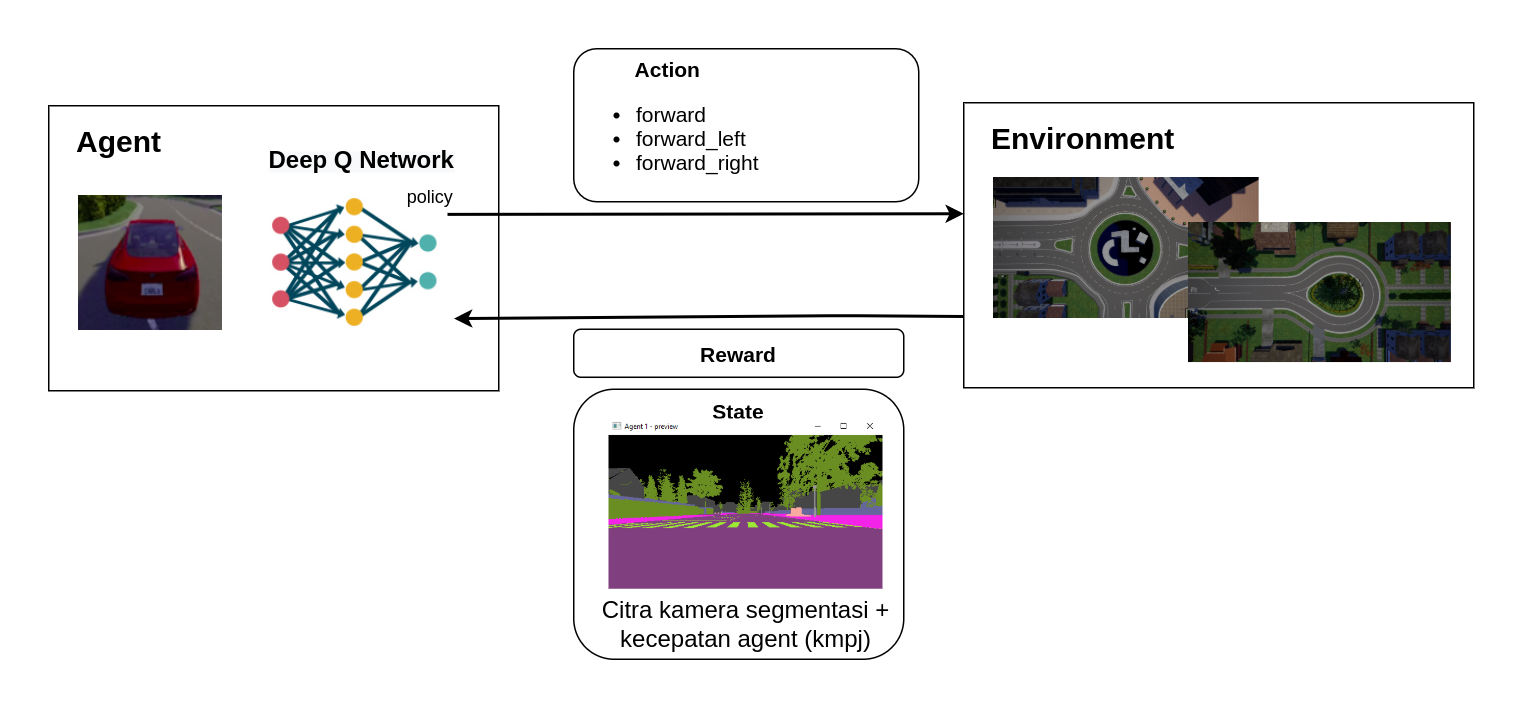
\includegraphics[width=1\linewidth]{images/metodologi}
	\caption{Diagram Blok Metodologi}
	\label{fig:blockdiagram}
\end{figure}

The training process is carried out after all configurations are completed. The training methodology of this research is shown in Figure \ref{fig:blockdiagram}. The agent in the simulation performs an action that causes the state to change. The state in the form of a segmentation image and agent speed (kmpj) as well as a reward from the agent is then sent to DQN for training. The result of the training in the form of a policy will determine the action which will then be carried out by the agent. Then the process will repeat itself into an endless cycle.

	
	
	
	\section{Testing and Result}
	\subsection{Training DQN}
	\label{sec:training_dqn}
	DQN algorithm training is carried out using the following hardware:
	\begin{table}[H]
		\begin{tabular}{ll}
			\textbf{CPU}  & Intel Core i5              \\
			\textbf{GPU}  & Nvidia GTX 1060 - 6GB VRAM \\
			\textbf{RAM}  & 8GB                        \\
			\textbf{Disk} & 256GB SSD M.2              \\
			\textbf{OS}   & Windows 10                
		\end{tabular}
		\caption{Hardware used for training.}
		\label{tb:hardwaresetup}
	\end{table}
	
	Training is done on a local machine using a GPU. The machine learning software environment used in training is:
	
	\begin{table}[H]
		\begin{tabular}{ll}
			\textbf{Software}  & \textbf{Version}              \\
			tensorflow-gpu  & 1.13.1	\\
			keras  & 2.2.5					\\
			h5py & 3.1              \\
			python & 3.7.9              \\
		\end{tabular}
		\caption{Software environment used for training.}
		\label{tb:softwaresetup}
	\end{table}
	
	
	The result of the training process is a DQN network model that represents an autonomous car movement planning system. The model is stored in a .model file format which can then be visualized with a tensorboard to see the results of the DQN algorithm training.
	
	\subsubsection{DQN training at Roundabout with Intersections using Grayscale Segmentation}
	\label{sec:training_dqn_bundaran_simpangempat_segmentasi_grayscale}
	
	The training of the DAN algorithm at the four-way roundabout with grayscale segmentation lasted for 20 hours. Here are the results of the DQN algorithm training visualization:
	
	\begin{figure}[H] 
		\centering
		\includegraphics[width=1\linewidth]{images/tensorboard_bundaran_simpangempat_segmentasi_grayscale}
		\caption{Tensorboard result on Roundabout with Intersections using Grayscale Segmentation}
		\label{fig:tensorboard_bundaran_simpangempat_segmentasi_grayscale}
	\end{figure}
	
	From the results of the DQN training visualization in Figure  \ref{fig:tensorboard_bundaran_simpangempat_segmentasi_grayscale}, it can be seen that the DQN algorithm training process has been running well. This can be seen from the value of accuracy, episode time, and rewards for driving autonomous cars which have an increasing trend as the training process progresses.
	
	\subsubsection{DQN training at Roundabout with Intersections using Advanced Segmentation}
	\label{sec:training_dqn_bundaran_simpangempat_segmentasi_hitam_putih}
	
	The DQN algorithm training at the four-way roundabout with advanced segmentation lasted for 13 hours, 30 minutes, and 48 seconds. Here are the results of the DQN algorithm training visualization:
	
	\begin{figure}[H] 
		\centering
		\includegraphics[width=1\linewidth]{images/tensorboard_bunderan_segmented}
		\caption{Tensorboard result on Roundabout with Intersections using Advanced Segmentation}
		\label{fig:tensorboard_bundaran_simpangempat_segmentasi_lanjutan}
	\end{figure}
	
	From the results of the DQN training visualization in Figure  \ref{fig:tensorboard_bundaran_tanpasimpang_segmentasi_lanjutan}, it can be seen that the DQN algorithm training process has been running well. This can be seen from the value of accuracy, episode time, and rewards for driving autonomous cars which have an increasing trend as the training process progresses.
	
	
	\subsubsection{DQN training at Roundabout without Intersections using Advanced Segmentation}
	\label{sec:training_dqn_bundaran_nosimpang_segmentasi_hitam_putih}
	
	DQN algorithm training on roundabouts without intersections with advanced segmentation lasted 26 hours and 25 seconds. The following are the results of the DQN algorithm training visualization:
	
	\begin{figure}[H] 
		\centering
		\includegraphics[width=1\linewidth]{images/tensorboard_itemputih_nosimpang}
		\caption{Tensorboard result on Roundabout without Intersections using Advanced Segmentation}
		\label{fig:tensorboard_bundaran_tanpasimpang_segmentasi_lanjutan}
	\end{figure}
	
	From the results of the DQN training visualization in Figure  \ref{fig:tensorboard_bundaran_tanpasimpang_segmentasi_lanjutan}, it can be seen that the DQN algorithm training process has been running well. This can be seen from the value of accuracy, episode time, and rewards for driving autonomous cars which have an increasing trend as the training process progresses.
	
	
	\subsection{DQN Model Test}
	\label{sec:pengujian_model_dqn}
	
	In this section, we will test the resulting model from the DQN training process. The test is carried out when the driving environment is under normal conditions.
	
	\subsubsection{DQN Model Test at Roundabout with Intersections using Grayscale Segmentation}
	\label{sec:pengujian_dqn_bundaran_simpangempat_segmentasi_grayscale}
	
	% Please add the following required packages to your document preamble:
	% \usepackage{graphicx}
	\begin{table}[H]
		\resizebox{\columnwidth}{!}{%
			\begin{tabular}{|l|l|l|l|l|}
				\hline
				episode\_length & avg\_speed & avg\_angle\_diff & avg\_dist\_diff & avg\_reward \\ \hline
				9.005           & 34.983     & 20.001           & 5.812           & 0.166       \\ \hline
				4.772           & 28.927     & 12.14            & 0.91            & 0.448       \\ \hline
				8.524           & 33.052     & 10.65            & 1.993           & 0.398       \\ \hline
				12.678          & 35.053     & 15.259           & 3.264           & 0.222       \\ \hline
				13.621          & 37.03      & 32.642           & 12.394          & 0.122       \\ \hline
				4.851           & 30.102     & 10.241           & 1.253           & 0.471       \\ \hline
				6.555           & 20.433     & 21.37            & 2.775           & 0.318       \\ \hline
				8.694           & 31.494     & 14.927           & 3.381           & 0.235       \\ \hline
				20.184          & 34.142     & 58.799           & 45.228          & -0.23       \\ \hline
				10.026          & 28.305     & 12.737           & 2.411           & 0.332       \\ \hline
				5.147           & 29.648     & 17.682           & 1.707           & 0.289       \\ \hline
				8.521           & 32.238     & 13.255           & 2.253           & 0.289       \\ \hline
				7.99            & 32.617     & 13.939           & 2.661           & 0.342       \\ \hline
				5.206           & 30.142     & 13.541           & 1.077           & 0.409       \\ \hline
				6.072           & 23.77      & 36.641           & 3.617           & 0.17        \\ \hline
				5.426           & 31.166     & 12.926           & 0.925           & 0.418       \\ \hline
				5.176           & 27.477     & 12.276           & 1.194           & 0.457       \\ \hline
				8.085           & 33.884     & 11.883           & 1.224           & 0.343       \\ \hline
				10.048          & 27.918     & 15.146           & 3.086           & 0.306       \\ \hline
				7.443           & 33.063     & 12.29            & 2.298           & 0.383       \\ \hline
				29.772          & 38.947     & 65.564           & 58.657          & -0.255      \\ \hline
				6.617           & 30.019     & 20.405           & 1.658           & 0.425       \\ \hline
				4.931           & 27.362     & 12.078           & 1.821           & 0.361       \\ \hline
				14.428          & 29.973     & 18.9             & 3.066           & 0.272       \\ \hline
				5.445           & 30.364     & 10.48            & 0.951           & 0.523       \\ \hline
				8.794           & 31.964     & 15.54            & 2.635           & 0.294       \\ \hline
				8.568           & 33.002     & 13.103           & 1.95            & 0.409       \\ \hline
				20.471          & 24.614     & 64.263           & 15.817          & -0.076      \\ \hline
				5.276           & 31.54      & 14.182           & 1.594           & 0.349       \\ \hline
				7.645           & 29.516     & 39.559           & 1.573           & 0.349       \\ \hline
			\end{tabular}%
		}
		\caption{30 result sample of DQN Model Test at Roundabout with Intersections using Grayscale Segmentation}
		\label{tb:hasilpengujian_bunderan_grayscale}
	\end{table}
	
	From the results of the sampling, conclusions are obtained as in table \ref{tb:kesimpulan_bunderan_grayscale}.
	
	% Please add the following required packages to your document preamble:
	% \usepackage{graphicx}
	\begin{table}[H]
		\resizebox{\columnwidth}{!}{%
			\begin{tabular}{|l|l|l|l|l|}
				\hline
				avg\_episode\_length & avg\_speed & avg\_angle\_diff & avg\_dist\_diff & avg\_reward \\ \hline
				9.332                & 30.758     & 21.413           & 6.306           & 0.284       \\ \hline
			\end{tabular}%
		}
		\caption{Summary of DQN Model Test at Roundabout with Intersections using Grayscale Segmentation}
		\label{tb:kesimpulan_bunderan_grayscale}
	\end{table}
	
	
	
	\subsubsection{DQN Model Test at Roundabout with Intersections using Advanced Segmentation}
	\label{sec:pengujian_dqn_bundaran_simpangempat_segmentasi_hitam_putih}
	
	\begin{table}[H]
		\resizebox{\columnwidth}{!}{%
			\begin{tabular}{|l|l|l|l|l|}
				\hline
				episode\_length & avg\_speed & avg\_angle\_diff & avg\_dist\_diff & avg\_reward \\ \hline
				7.431           & 38.229     & 10.205           & 2.0             & 0.34        \\ \hline
				8.094           & 30.83      & 24.743           & 1.187           & 0.392       \\ \hline
				8.418           & 30.337     & 20.039           & 2.106           & 0.257       \\ \hline
				21.587          & 37.044     & 14.712           & 2.588           & 0.28        \\ \hline
				7.019           & 35.495     & 11.015           & 0.849           & 0.465       \\ \hline
				19.252          & 35.029     & 20.848           & 3.259           & 0.267       \\ \hline
				18.607          & 29.382     & 58.62            & 6.881           & 0.071       \\ \hline
				6.529           & 36.715     & 10.4             & 1.301           & 0.348       \\ \hline
				14.337          & 36.066     & 16.105           & 0.99            & 0.421       \\ \hline
				17.025          & 34.249     & 45.883           & 4.252           & 0.15        \\ \hline
				9.511           & 41.363     & 12.647           & 1.503           & 0.32        \\ \hline
				36.864          & 34.917     & 68.418           & 8.128           & 0.069       \\ \hline
				9.973           & 38.902     & 13.901           & 1.56            & 0.304       \\ \hline
				7.34            & 35.594     & 13.333           & 1.547           & 0.45        \\ \hline
				14.864          & 31.482     & 59.456           & 3.588           & 0.112       \\ \hline
				9.987           & 41.68      & 12.595           & 1.952           & 0.297       \\ \hline
				9.767           & 39.018     & 15.001           & 1.341           & 0.373       \\ \hline
				7.011           & 36.749     & 10.62            & 1.488           & 0.321       \\ \hline
				17.4            & 26.631     & 79.254           & 13.336          & -0.07       \\ \hline
				12.798          & 40.187     & 15.749           & 1.645           & 0.285       \\ \hline
				17.809          & 31.448     & 46.125           & 2.951           & 0.268       \\ \hline
				11.504          & 36.149     & 21.827           & 1.347           & 0.355       \\ \hline
				6.395           & 37.127     & 9.601            & 0.895           & 0.418       \\ \hline
				23.591          & 30.945     & 60.991           & 4.07            & 0.153       \\ \hline
				6.957           & 37.284     & 8.505            & 0.959           & 0.438       \\ \hline
				9.431           & 40.093     & 11.436           & 1.98            & 0.311       \\ \hline
				35.604          & 27.912     & 80.507           & 11.311          & -0.171      \\ \hline
				9.089           & 42.26      & 10.891           & 1.286           & 0.395       \\ \hline
				7.032           & 36.387     & 11.418           & 1.278           & 0.418       \\ \hline
				8.578           & 34.796     & 15.489           & 1.456           & 0.316       \\ \hline
			\end{tabular}%
		}
		\caption{30 result sample of DQN Model Test at Roundabout with Intersections using Advanced Segmentation}
		\label{tb:hasilpengujian_bunderan_segmented}
	\end{table}
	
	From the results of the sampling, conclusions are obtained as in table \ref{tb:kesimpulan_bunderan_segmented}.
	
	
	% Please add the following required packages to your document preamble:
	% \usepackage{graphicx}
	\begin{table}[H]
		\resizebox{\columnwidth}{!}{%
			\begin{tabular}{|l|l|l|l|l|}
				\hline
				avg\_episode\_length & avg\_speed & avg\_angle\_diff & avg\_dist\_diff & avg\_reward \\ \hline
				13.326                & 35.476     & 27.011           & 2.967           & 0.278       \\ \hline
			\end{tabular}%
		}
		\caption{Summary of DQN Model Test at Roundabout with Intersections using Advanced Segmentation}
		\label{tb:kesimpulan_bunderan_segmented}
	\end{table}
	
	\subsubsection{DQN Model Test at Roundabout without Intersections using Advanced Segmentation}
	\label{sec:pengujian_dqn_bundaran_nosimpang_segmentasi_hitam_putih}
	
	\begin{table}[H]
		\begin{tabular}{|l|l|l|l|}
			\hline
			episode\_length & avg\_speed  & avg\_alpha  & avg\_reward \\ \hline
			8.374           & 32.202 & 31.098 & 0.113  \\ \hline
			8.796           & 29.909 & 32.023 & 0.093  \\ \hline
			12.195          & 29.678 & 40.528 & 0.068  \\ \hline
			12.439          & 30.384 & 36.557 & 0.12   \\ \hline
			10.246          & 29.72  & 42.027 & 0.063  \\ \hline
			3.138           & 19.86  & 32.557 & 0.085  \\ \hline
			9.982           & 30.777 & 35.319 & 0.129  \\ \hline
			8.185           & 30.64  & 24.322 & 0.112  \\ \hline
			9.719           & 31.814 & 31.563 & 0.081  \\ \hline
			10.908          & 33.314 & 38.641 & 0.097  \\ \hline
			3.299           & 21.882 & 22.22  & 0.122  \\ \hline
			9.27            & 31.347 & 26.635 & 0.12   \\ \hline
			4.27            & 26.317 & 16.402 & 0.152  \\ \hline
			3.765           & 23.032 & 32.14  & 0.169  \\ \hline
			10.776          & 31.581 & 37.949 & 0.091  \\ \hline
			5.588           & 28.784 & 29.461 & 0.155  \\ \hline
			3.219           & 22.536 & 20.392 & 0.186  \\ \hline
			8.508           & 30.489 & 24.669 & 0.122  \\ \hline
			4.457           & 23.68  & 23.546 & 0.146  \\ \hline
			3.824           & 22.575 & 36.989 & 0.105  \\ \hline
			10.599          & 31.869 & 23.992 & 0.132  \\ \hline
			12.438          & 31.08  & 38.071 & 0.088  \\ \hline
			7.873           & 31.305 & 21.448 & 0.15   \\ \hline
			3.562           & 22.864 & 16.225 & 0.136  \\ \hline
			8.758           & 27.877 & 37.786 & 0.076  \\ \hline
			4.641           & 26.732 & 25.345 & 0.106  \\ \hline
			10.472          & 32.074 & 33.322 & 0.101  \\ \hline
			10.937          & 31.784 & 33.864 & 0.095  \\ \hline
			9.244           & 30.508 & 28.196 & 0.12   \\ \hline
		\end{tabular}
		\caption{30 result sample of DQN Model Test at Roundabout without Intersections using Advanced Segmentation}
		\label{tb:hasilpengujian_notbunderan_segmented}
	\end{table}
	
	From the results of the sampling, conclusions are obtained as in table \ref{tb:kesimpulan_notbunderan_segmented}.
	
	% Please add the following required packages to your document preamble:
	% \usepackage{graphicx}
	\begin{table}[H]
		\resizebox{\columnwidth}{!}{%
			\begin{tabular}{|l|l|l|l|}
				\hline
				avg\_episode\_length & avg\_speed & avg\_alpha & avg\_reward \\ \hline
				7.958                & 28.533     & 30.068     & 0.115       \\ \hline
			\end{tabular}%
		}
		\caption{Summary of DQN Model Test at Roundabout without Intersections using Advanced Segmentation}
		\label{tb:kesimpulan_notbunderan_segmented}
	\end{table}
	
	
	\section{Conclusion}
	\vspace{1ex}
	
	\subsection{Conclusion}
	\label{sec:kesimpulan}
	
	From the system design and testing that has been done, some conclusions are obtained as follows. The constraints and shortcomings that the authors face are also written in the suggestions section in the hope of assisting the development of further research.
	
	\begin{enumerate}
		
		\item The autonomous car movement planning system based on the DQN algorithm which is designed to be able to accelerate and steer, is able to control the autonomous car and understand the surrounding conditions.
		
		\item Use of image state with advanced segmentation; ie producing drivable and non-drivable image outputs produces better results than ordinary segmentation with 42.8\% better average episode length performance, 15.3\% better average speed, and 112.4\% better average distance difference.
		
	\end{enumerate}
	
	\subsection{Suggestion}
	\label{chap:saran}
	
	For further development on the topic of autonomous car movement planning research using the DQN algorithm, there are several suggestions given, including the following:
	
	\begin{enumerate}
		
		\item The sensors used for navigation from agents using the DQN algorithm can be added to more such as GPS and LIDAR, so that agents can act with more complete parameters.
		
		\item The training process can be carried out with a longer time and using machines with stronger computing power in order to obtain a convergent model.
	\end{enumerate}
	
	\bibliographystyle{IEEEtran}
	\bibliography{dpustaka}
\end{document}
